\documentclass[12pt]{article}
\usepackage[utf8]{inputenc}
\usepackage{amsmath}
\usepackage{amssymb}
\usepackage{geometry}
\usepackage{microtype}
\usepackage{ragged2e}
\usepackage{tikz}
\usepackage{graphicx}
\usepackage{svg}
\usepackage{newtxtext}
\usepackage{newtxmath}
\geometry{margin=1in}
\setlength{\parindent}{0pt}
\setlength{\parskip}{0.25em}

\begin{document}
\justifying

\begin{titlepage}
\centering
\vspace*{0.5in}
\begin{minipage}[t]{0.25\textwidth}
\centering

\includegraphics[height=1.2in]{../figures/Cairo_University_Crest.png}
\end{minipage}
\begin{minipage}[t]{0.45\textwidth}
\centering

\includegraphics[height=1.2in]{../figures/AER.png}
\end{minipage}
\begin{minipage}[t]{0.25\textwidth}
\centering

\includegraphics[height=1.2in]{../figures/UNI.png}
\end{minipage}

\vspace{0.6in}
{\LARGE Graduation Project\par}
\vspace{0.25in}
{\Large 2D Laplace Problem with Dirichlet Boundary Conditions\par}
\vspace{0.3in}
\rule{0.75\textwidth}{0.6pt}
\vspace{0.4in}

\vfill
\end{titlepage}

\clearpage

\tableofcontents

\clearpage

\section{Problem Description}
This project solves a steady 2D diffusion problem on a unit square using a high-order finite element method. There are no source terms, so it is a simple test used to check accuracy as the mesh is refined and the polynomial order increases.

The domain is a unit square in the $x$--$y$ plane. The boundary condition on the bottom edge is a sine curve, and the other three edges are set to zero. The boundary data are shown below.

\begin{figure}[h]
\centering
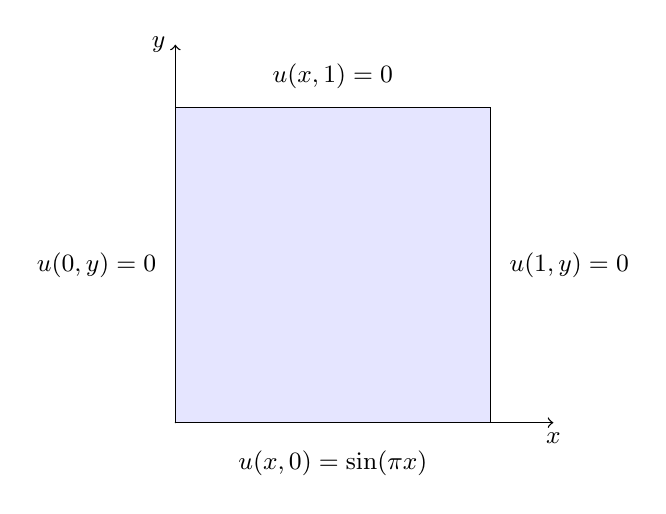
\begin{tikzpicture}[scale=4.0, line cap=round, every node/.style={font=\small}]
	% axes
	\draw[->, line width=0.5pt] (0,0) -- (1.2,0) node[below] {$x$};
	\draw[->, line width=0.5pt] (0,0) -- (0,1.2) node[left] {$y$};
	% unit square
	\fill[blue!10] (0,0) rectangle (1,1);
	\draw[line width=0.6pt] (0,0) rectangle (1,1);
	% boundary data
	\node[above] at (0.5,1.03) {$u(x,1)=0$};
	\node[right] at (1.03,0.5) {$u(1,y)=0$};
	\node[left] at (-0.03,0.5) {$u(0,y)=0$};
	\node[below] at (0.5,-0.06) {$u(x,0)=\sin(\pi x)$};
\end{tikzpicture}
\caption{Unit square domain and Dirichlet boundary data.}
\end{figure}

The governing equation is the Laplace equation
\begin{equation}
\nabla^2 u = 0 \quad \text{in } [0,1] \times [0,1].
\end{equation}

The Dirichlet boundary conditions are
\begin{align}
u(x,0) &= \sin(\pi x), \\
u(x,1) &= 0, \\
u(0,y) &= 0, \\
u(1,y) &= 0.
\end{align}

This boundary value problem has the exact closed-form solution
\begin{equation}
u(x,y) = \big(\cosh(\pi y) - \coth(\pi)\,\sinh(\pi y)\big)\,\sin(\pi x),
\end{equation}
which is used to compute the $L^2$ and $H^1$ error norms for verification.

\clearpage
\section{Numerical Method}
\subsection{Weak Formulation}
We start with the residual
\begin{equation}
R = \frac{\partial^2 u}{\partial x^2} + \frac{\partial^2 u}{\partial y^2},
\end{equation}
and choose the weight $W = N_i$. The weighted residual statement is
\begin{equation}
\iint_{\Omega} R\, W\, d\Omega = \iint_{\Omega} \left( \frac{\partial^2 u}{\partial x^2} + \frac{\partial^2 u}{\partial y^2} \right) N_i\, d\Omega = 0.
\end{equation}
After integration by parts we get
\begin{equation}
\iint_{\Omega} \left( \frac{\partial u}{\partial x}\, \frac{\partial N_i}{\partial x} + \frac{\partial u}{\partial y}\, \frac{\partial N_i}{\partial y} \right) d\Omega
- \int_{\Gamma} N_i\, \nabla u \cdot \mathbf{n}\, d\Gamma = 0.
\end{equation}
We apply Dirichlet values directly, so the boundary term is zero.

\subsection{Finite Element Approximation}
We start from the Laplace equation and the weighted residual statement. In compact form,
\begin{equation}
\frac{\partial^2 u}{\partial x^2} + \frac{\partial^2 u}{\partial y^2} = 0, \qquad
\iint_{\Omega} \left( \frac{\partial^2 u}{\partial x^2} + \frac{\partial^2 u}{\partial y^2} \right) N_i\, d\Omega = 0.
\end{equation}
After integration by parts, the weak form becomes
\begin{equation}
\iint_{\Omega} \left( \frac{\partial u}{\partial x}\, \frac{\partial N_i}{\partial x} + \frac{\partial u}{\partial y}\, \frac{\partial N_i}{\partial y} \right) d\Omega
- \int_{\Gamma} N_i\, \nabla u \cdot \mathbf{n}\, d\Gamma = 0.
\end{equation}

We approximate the solution inside one element by
\begin{equation}
u_h = \sum_{j=1}^{n_e} N_j u_j, \qquad
u_{h,x} = \sum_{j=1}^{n_e} \frac{\partial N_j}{\partial x} u_j, \qquad
u_{h,y} = \sum_{j=1}^{n_e} \frac{\partial N_j}{\partial y} u_j.
\end{equation}
Substituting gives the local matrix form
\begin{equation}
\sum_{j=1}^{n_e} \left[ \iint_{\Omega_e} \left( \frac{\partial N_i}{\partial x}\, \frac{\partial N_j}{\partial x} + \frac{\partial N_i}{\partial y}\, \frac{\partial N_j}{\partial y} \right) d\Omega \right] u_j = 0,
\end{equation}
or, in matrix notation,
\begin{equation}
\mathbf{K}_e \mathbf{u}_e = \mathbf{0}, \qquad
\mathbf{K}_e = \iint_{\Omega_e} \left( \mathbf{N}_x^T \mathbf{N}_x + \mathbf{N}_y^T \mathbf{N}_y \right) d\Omega.
\end{equation}

\subsection{Spatial Discretization}

The domain is the unit square $[0,1] \times [0,1]$ and it is split into structured quadrilateral elements. We use Q$p$ elements (polynomial order $p$) for the solution, and the geometry order can be set to $p_G$ (isoparametric when $p_G=p$).

The global system assembled is
\begin{equation}
\mathbf{K} \mathbf{u} = \mathbf{f},
\end{equation}
where the element stiffness matrix is
\begin{equation}
K_e = \iint_{\Omega_e} \left( \frac{\partial N}{\partial x}^T \frac{\partial N}{\partial x} + \frac{\partial N}{\partial y}^T \frac{\partial N}{\partial y} \right) d\Omega.
\end{equation}

\subsection{Numerical Quadrature and Mapping}
Gauss--Legendre quadrature is used to evaluate element integrals. Shape function derivatives are computed in reference coordinates and mapped to physical coordinates through the Jacobian of the isoparametric transformation. The determinant of the Jacobian scales the integration weights.

\subsection{Boundary Conditions}
Dirichlet boundary conditions are enforced by directly modifying the global system: rows corresponding to boundary nodes are zeroed and set to identity, with the right-hand side set to the prescribed value. This imposes the boundary values strongly.

\clearpage

\section{Error Norms}
\subsection{Computation of Error Norms}
To quantify accuracy, we compare the numerical solution against the exact solution using standard $L^2$ and $H^1$ norms. These measures capture the overall error and the error in gradients, which is important for a diffusion problem. The expressions below follow the same quadrature procedure used in the stiffness matrix assembly. This keeps the verification consistent with the discretization.

For the $L^2$ norm, starting from the definition,
\begin{align}
\lVert u-u_h \rVert_{L^2(\Omega)}
&= \sqrt{ \iint_{\Omega} (u-u_h)^2\, d\Omega } \\
&= \sqrt{ \sum_{k} \int_{\Omega_k} (u-u_h)^2\, d\Omega } \\
&\approx \sqrt{ \sum_{k} \sum_{g} \left[(u-u_h)^2\right]_{x_g}\, w_g\, |J|_g }.
\end{align}

For the $H^1$ norm, starting from the definition and adding the gradient mismatch,
\begin{align}
\lVert u-u_h \rVert_{H^1(\Omega)}
&= \sqrt{ \iint_{\Omega} \left[(u-u_h)^2 + \lVert \nabla u - \nabla u_h \rVert^2\right] d\Omega } \\
&= \sqrt{ \iint_{\Omega} \left[(u-u_h)^2 + (u_x-u_{h,x})^2 + (u_y-u_{h,y})^2\right] d\Omega } \\
&= \sqrt{ \sum_{k} \int_{\Omega_k} \left[(u-u_h)^2 + (u_x-u_{h,x})^2 + (u_y-u_{h,y})^2\right] d\Omega } \\
&\approx \sqrt{ \sum_{k} \sum_{g} \left[(u-u_h)^2 + (u_x-u_{h,x})^2 + (u_y-u_{h,y})^2\right]_{x_g}\, w_g\, |J|_g }.
\end{align}
Here $u_h$ is the finite element solution, $u$ is the exact solution, and $u_x$ and $u_y$ are the exact derivatives. From
\begin{equation}
u(x,y) = \big(\cosh(\pi y) - \coth(\pi)\,\sinh(\pi y)\big)\,\sin(\pi x),
\end{equation}
the exact derivatives are
\begin{align}
u_x(x,y) &= \pi\,\big(\cosh(\pi y) - \coth(\pi)\,\sinh(\pi y)\big)\,\cos(\pi x),\\
u_y(x,y) &= \pi\,\big(\sinh(\pi y) - \coth(\pi)\,\cosh(\pi y)\big)\,\sin(\pi x).
\end{align}

\subsection{Theoretical Error Estimates}
Theoretically, for sufficiently smooth solutions and regular meshes, the finite element error in the $L^2$ and $H^1$ norms behaves as:
\begin{align}
\lVert u-u_h \rVert_{L^2(\Omega)} &\leq C_1\, h^{p+1}, \\
\lVert u-u_h \rVert_{H^1(\Omega)} &\leq C_2\, h^{p},
\end{align}

where,
\begin{itemize}
	\item $h$ is the characteristic mesh size.
	\item $p$ is the polynomial degree of the finite element basis functions.
	\item $C_1$ and $C_2$ are constants that do not depend on $h$.
\end{itemize}
For a uniform mesh of $N$ elements in two dimensions, 
\begin{align}
h = 1/\sqrt{N}.
\end{align}

These estimates show that as the mesh is refined (i.e., as $h$ decreases) or as the polynomial degree $p$ increases, the error in the $L^2$ norm decreases at a rate proportional to $h^{p+1}$, and the error in the $H^1$ norm decreases at a rate proportional to $h^p$.
\clearpage
\section{Results and Discussion}
\subsection{Mesh}
Figure~\ref{fig:mesh_updated} shows the structured mesh used in the study. The nodal distribution is uniform and aligned with the Cartesian boundaries, which is appropriate for this smooth solution and enables a clean assessment of convergence with respect to $h$ and $p$.

\begin{figure}[htbp]
\centering
\includesvg[width=0.95\textwidth]{../figures/Mesh}
\caption{structured quadrilateral mesh for the unit square.}
\label{fig:mesh_updated}
\end{figure}

\clearpage

\subsection{Numerical and Exact Solutions}
Figure~\ref{fig:uh_field} presents the numerical solution computed using a 36-element mesh with Q4 geometry and a Q16 solution basis. Figure~\ref{fig:exact_field} presents the exact solution used for verification.

\begin{figure}[htbp]
\centering
\includesvg[width=0.8\textwidth]{../figures/FEMSolution}
\caption{Finite element solution $u_h(x,y)$ on the unit square.}
\label{fig:uh_field}
\end{figure}

\begin{figure}[htbp]
\centering
\includesvg[width=0.8\textwidth]{../figures/Exact}
\caption{Exact solution $u(x,y)$ used for verification.}
\label{fig:exact_field}
\end{figure}

\clearpage

\subsection{3D Surface View}
The 3D surface view in Figure~\ref{fig:uh_surface} confirms the smooth exponential decay in $y$ combined with the sinusoidal variation in $x$, matching the analytic form of the solution.

\begin{figure}[htbp]
\centering
\includesvg[width=0.95\textwidth]{../figures/3DImage}
\caption{3D surface plot of the finite element solution.}
\label{fig:uh_surface}
\end{figure}

\clearpage

\subsection{Pointwise Comparison}
Figure~\ref{fig:line_compare} compares the numerical and exact solutions along the line $x=0.5$. The two curves overlap closely across the domain, indicating that the discretization accurately captures both amplitude and phase of the sinusoidal mode, with the largest deviations near the boundaries where gradients are strongest.

\begin{figure}[htbp]
\centering
\includesvg[width=0.95\textwidth]{../figures/comparisonAlongHalfX}
\caption{Comparison of numerical and exact solutions along $x=0.5$.}
\label{fig:line_compare}
\end{figure}

\clearpage

\subsection{Isoparametric Norms}
\subsubsection{$L^2$ Norm}
Figure~\ref{fig:l2_iso} shows the $L^2$ convergence history for the isoparametric case ($p_G=p$). The error decreases with mesh refinement and with increasing polynomial order, which matches the expected convergence for a smooth solution. The runtime shown in the plot title is 154 s.

\begin{figure}[htbp]
\centering
\includesvg[width=1.0\textwidth]{../figures/L2NormIsoparametricCorected}
\caption{$L^2$ error convergence for the isoparametric case.}
\label{fig:l2_iso}
\end{figure}

\clearpage

\subsubsection{$H^1$ Norm}
Figure~\ref{fig:h1_iso} shows the $H^1$ convergence history for the isoparametric case. The trend is consistent with optimal convergence for this smooth problem.

\begin{figure}[htbp]
\centering
\includesvg[width=1.0\textwidth]{../figures/H1NormIsoparametricCorected}
\caption{$H^1$ error convergence for the isoparametric case.}
\label{fig:h1_iso}
\end{figure}

\clearpage

\subsection{Subparametric Norms}
\subsubsection{$L^2$ Norm}
Figure~\ref{fig:l2_sub} shows the $L^2$ convergence history for the subparametric geometry case. The runtime shown in the plot title is 42 s, which is lower than the isoparametric case (154 s).

\begin{figure}[htbp]
\centering
\includesvg[width=1.0\textwidth]{../figures/L2NormsubparametricCorected}
\caption{$L^2$ error convergence for the subparametric geometry case.}
\label{fig:l2_sub}
\end{figure}

\clearpage

\subsubsection{$H^1$ Norm}
Figure~\ref{fig:h1_sub} shows the $H^1$ convergence history for the subparametric geometry case. The gradient error reflects the geometry under-resolution in this configuration.

\begin{figure}[htbp]
\centering
\includesvg[width=1.0\textwidth]{../figures/H1NormsubparametricCorected}
\caption{$H^1$ error convergence for the subparametric geometry case.}
\label{fig:h1_sub}
\end{figure}

Overall, the results confirm that the solver reproduces the analytic solution accurately, with clear convergence in both $L^2$ and $H^1$ norms. The relative behavior of the isoparametric and subparametric cases can be compared directly in Figures~\ref{fig:l2_iso}--\ref{fig:h1_sub}.
\clearpage
\subsection{h-refinement vs p-refinement}

Figure~\ref{fig:h_vs_p} shows the $L^2$ error convergence history for 
h-refinement using first-order elements and p-refinement performed on 
the coarsest mesh. The error is plotted against the number of degrees 
of freedom on a log--log scale.

\begin{figure}[htbp]
\centering
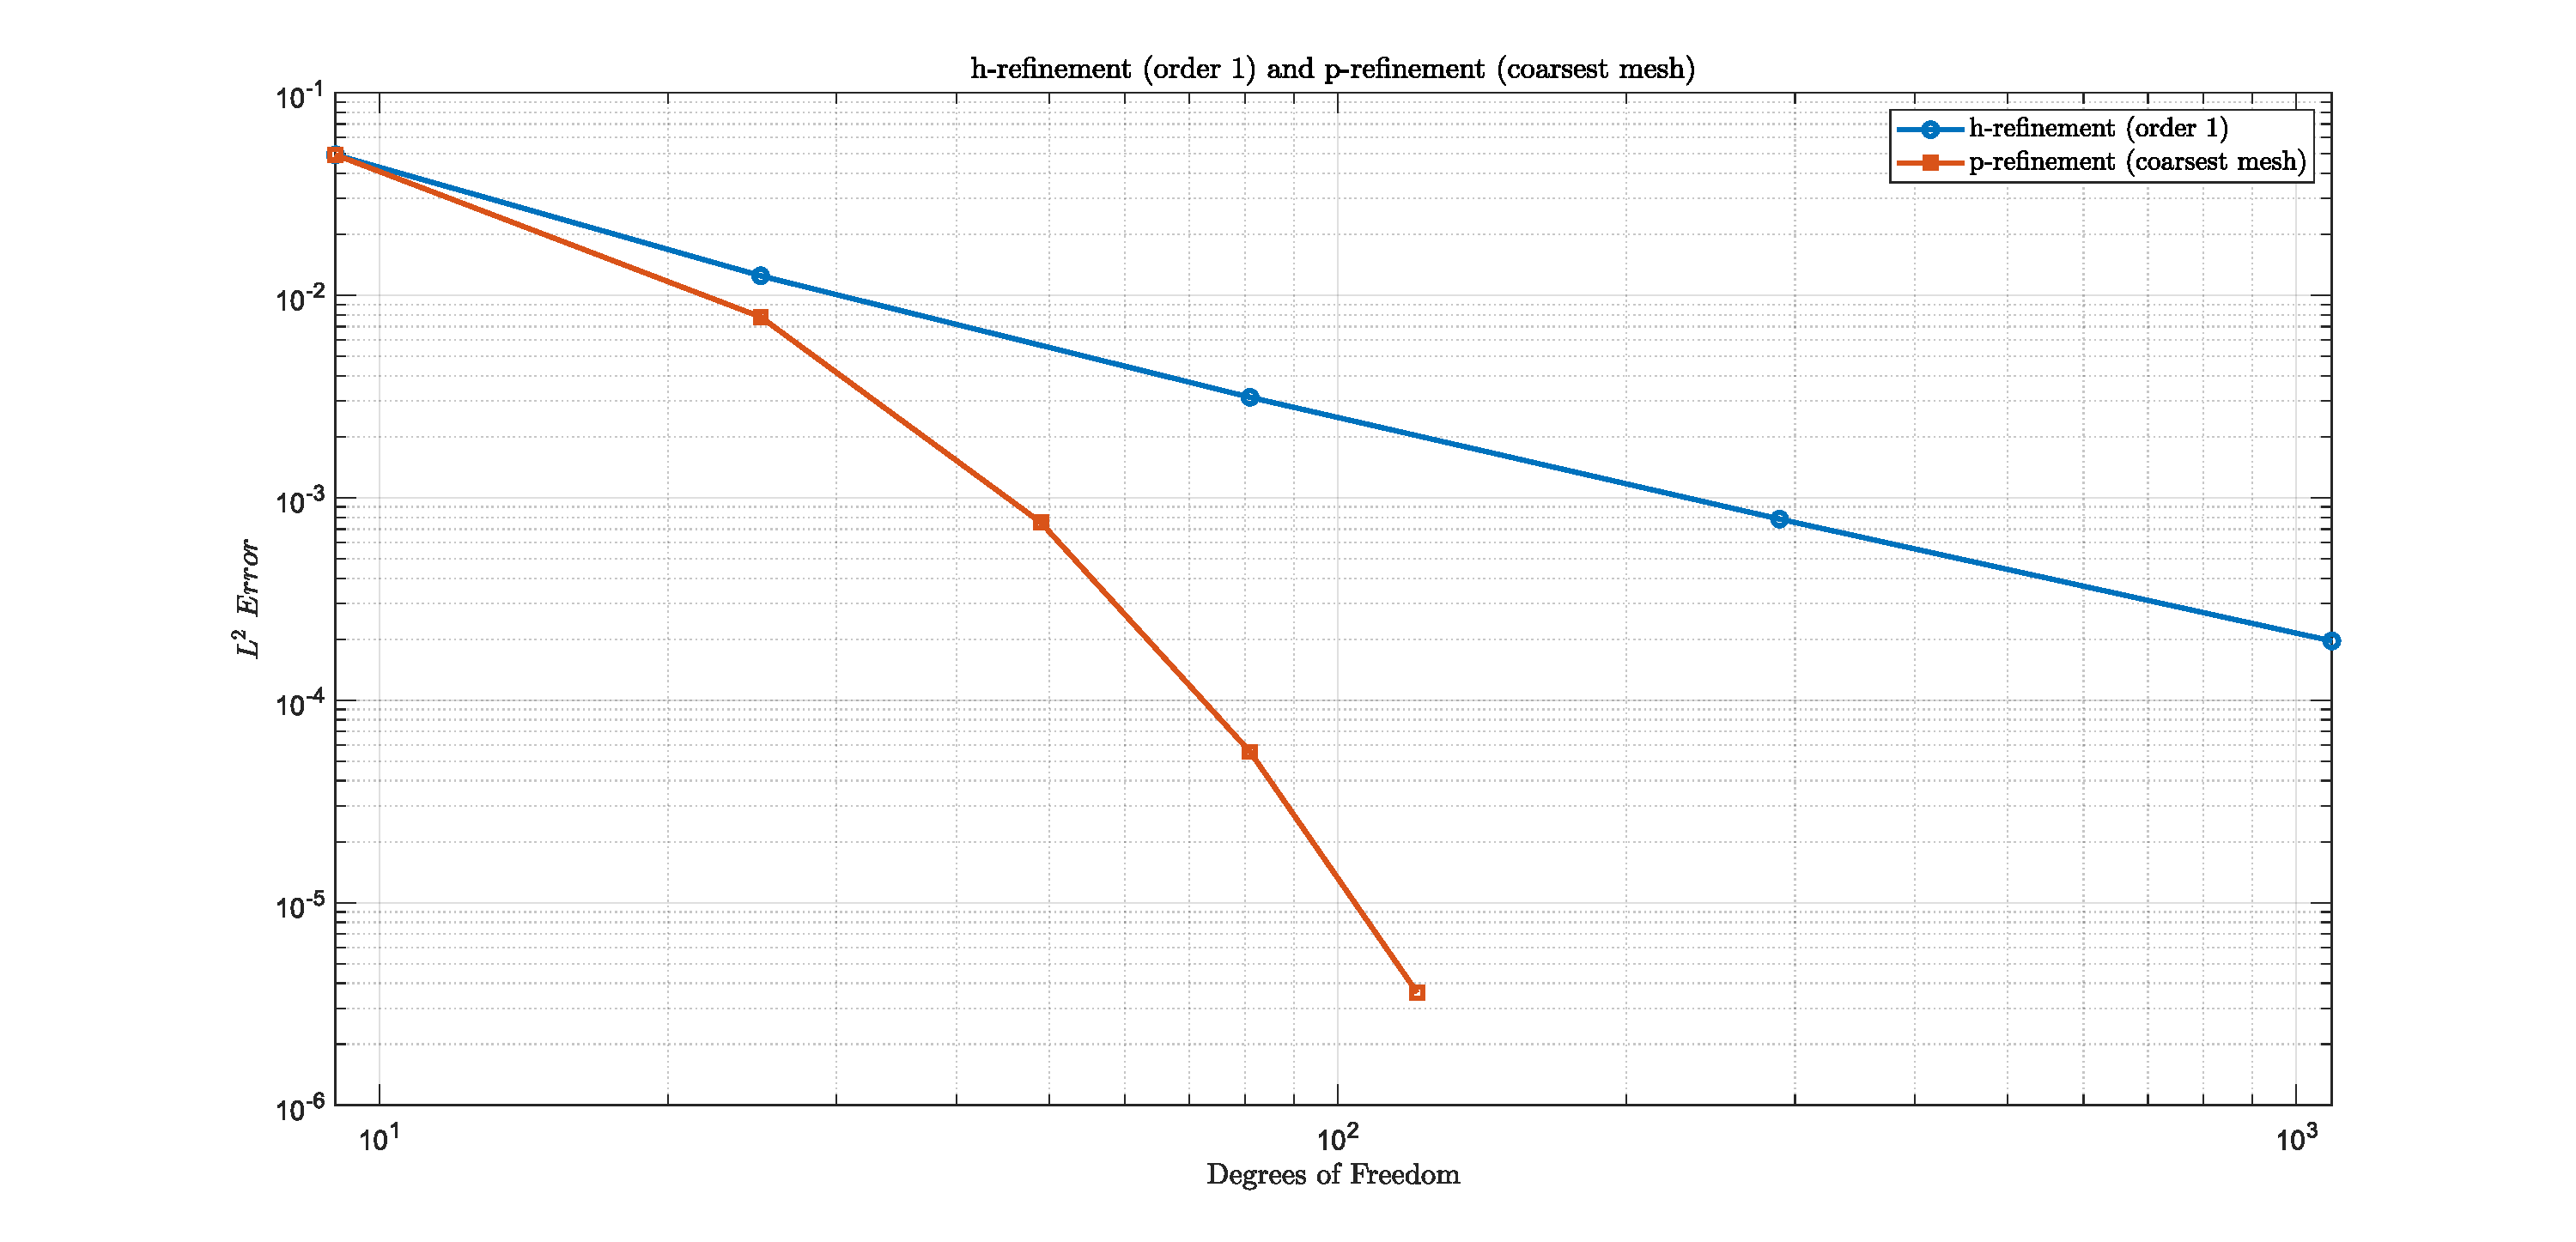
\includegraphics[width=1.0\textwidth]{../figures/ISOHvsP}
\caption{$L^2$ error convergence for h-refinement and 
p-refinement.}
\label{fig:h_vs_p}
\end{figure}

\end{document}